
\section{Graphs \& Manifolds}

\begin{frame}{Graph - Definitions}

  \begin{block}{Graph Definition}
    A graph is defined as $G = \langle V,E \rangle$, where $V$ is a set of 
    nodes and $E$ is a set of edges. 
  \end{block}

  \pause

  \begin{columns}
    \column{.55\textwidth}

    \begin{block}{Nodes}
      $(n_1, n_2, \dots) \in \mathbb{R}^F$, with $F$ as node feature dimensions.
    \end{block}
  
    \begin{block}{Edges}
      Edges are defined as a set of tuples $(i, j)$, where $i$ and $j$ determine 
      the index of the nodes.
    \end{block}

    \column{.45\textwidth}
    \begin{figure}
      \centering
      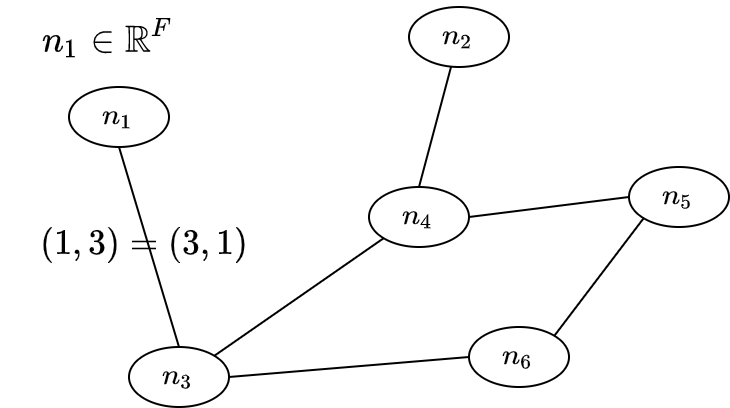
\includegraphics[width=\textwidth]{graph_undirected.drawio.png}
      \caption{Sample graph}        
    \end{figure}
  \end{columns}


  \begin{figure}
    
  \end{figure}

\end{frame}

\begin{frame}{Graph - Definitions - Adjacency Matrix}
\begin{columns}
  \column{.55\textwidth}

  \begin{block}{Adjacency Matrix}
    The binary adjacency matrix of graph $G = \langle V, E \rangle$ is defined as:
  \begin{equation}
      \label{eg:AdjacencyMatrix}
      A_{ij} =    
      \begin{cases}
          1  & \text{if } (i, j) \in E \\
          0, & \text{otherwise}
      \end{cases}
  \end{equation}
  \end{block}

  \pause
  
  \column{.45\textwidth}
  \begin{figure}
    \centering
    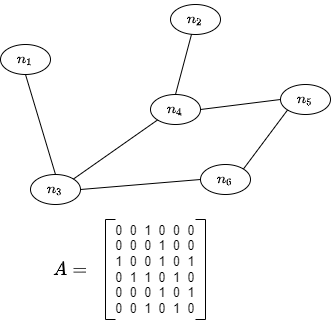
\includegraphics[width=0.9\textwidth]{graph_A.drawio.png}
    \caption{Sample graph}        
  \end{figure}

\end{columns}

\end{frame}

\begin{frame}{Graph - Definitions - Degree}
  \begin{columns}
    \column{.55\textwidth}
  
    \begin{block}{Degree of a node}
      The $degree$ of a node is defined as the number of (incoming) edges.
    \end{block}

    \begin{block}{Degree Matrix of Graph $G$}
      Is a diagonal matrix with degree of nodes as entries.
      $$D_{ii} = degree(n_i)$$
    \end{block}
  
    \pause

    \column{.45\textwidth}
    \begin{figure}
      \centering
      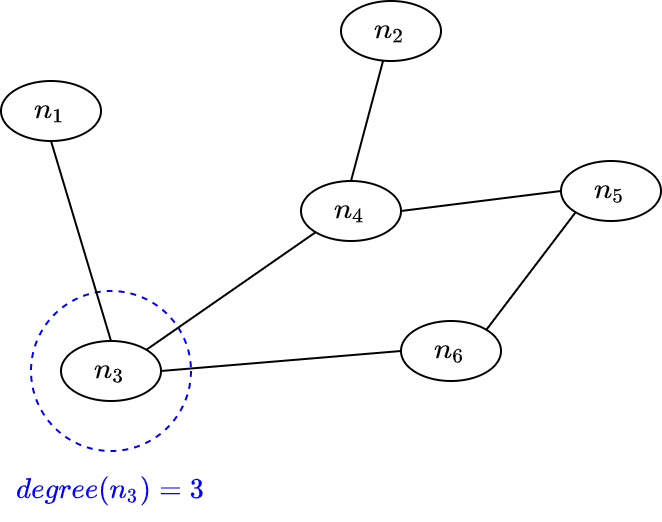
\includegraphics[width=0.9\textwidth]{graph_degree.drawio.png}
      \caption{Sample graph}        
    \end{figure}
  
  \end{columns}
  
  \end{frame}

\begin{frame}{Graph for Molecular Imaging Observation}
  \begin{columns}
    \column{0.45\textwidth}
    \begin{itemize}
      \item Nodes: Single observation $y_i$
      \item Edges: Use k-nearest neighbours (k-NN) to construct a graph
      \item Define similarity measure:
      
    \end{itemize}

    \column{0.55\textwidth}
    \pause
    \begin{figure}
      \centering
      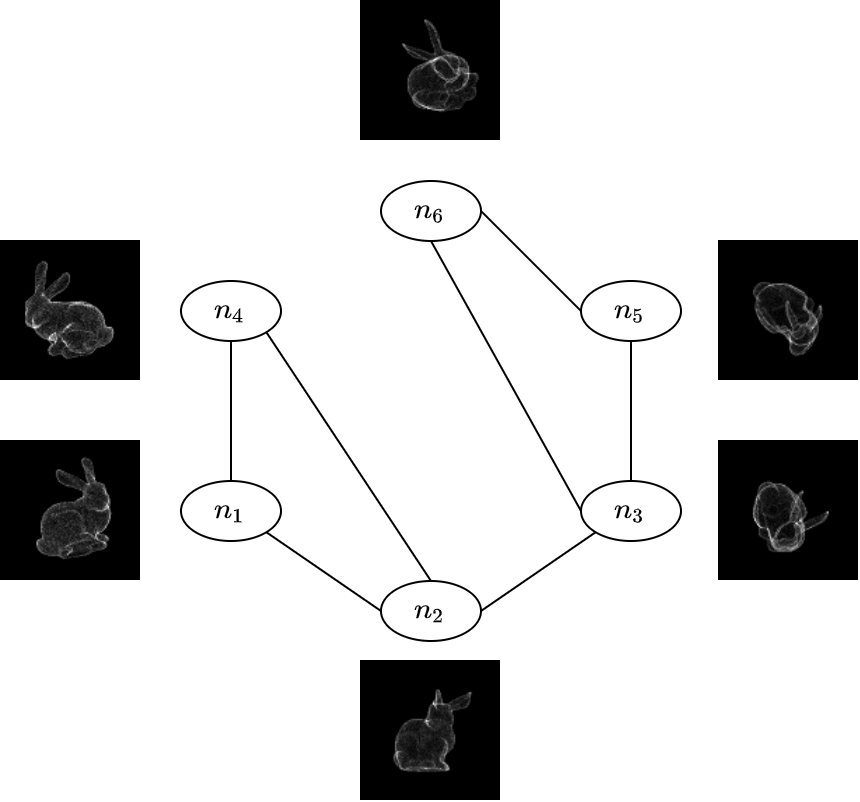
\includegraphics[width=0.8\textwidth]{cryo-EM_graph.drawio.png}
      \caption{Sample graph for cryo-EM observation}        
    \end{figure}
  

  \end{columns}
\end{frame}


\begin{frame}{Graph Laplacian (GL)}
\begin{itemize}
  \item What can we use this graph for?
  \item \cite{LaplaceRandomProjections} used it to approximate angles:
\end{itemize}

\begin{block}{Low-dimensional Embedding}
  \begin{enumerate}
    \item Construct a k-NN graph from observations.
    \item Calculate $L = D - A $
    \item Get 2nd and 3rd smallest eigenvalue with corresponding eigenvectors.
  \end{enumerate}
\end{block}

\end{frame}

%\begin{frame}[c]{Noisy graph}
%
%    \begin{definition}
%        For every noisy graph $G_0 = \langle V, E_0 \rangle$, 
%        there exists a noiseless graph $G = \langle V, E \rangle$.
%        Both graphs consists of the same set of vertices $V$ but different edges.
%        $E_0$  is defined as follows:
%        $$E_0 = E \setminus  E^{-}_0 \cup  E^{+}_0,$$
%        where $E^{-}_0 \subseteq E$ and $E^{+}_0 \subseteq U$ with $U$ the set of all possible edges and $E^{+}_0 \cap E = \emptyset$
%    \end{theorem}
%
%\end{frame}

\begin{frame}{Low\-dimensional Embedding}

  some notes and show clean embedding
  
\end{frame}


\begin{frame}{Unknown angles}
  Show reconstruction with calculated angles
\end{frame}
  

\begin{frame}{High-noise domain}

  Show graph
  Show embedding
  Show reconstruction

\end{frame}



\begin{frame}[c]{Graph Denoising}
    \textit{Graph denoising} is the task, to estimate a denoised graph $\tilde{G}$  
    from a given noisy graph $G_0$, with underlying original graph $G$:

    \begin{definition}[Graph Denoising]
        $$GD: G_0 \mapsto \tilde{G} \approx G,$$
    \end{definition}
    where $G_0$, $\tilde{G}$, $G$ denotes noisy, estimated denoised and original graph respectively.
\end{frame}

\begin{frame}{Traditional Denoising}

  BM3D
  Non-local means
\end{frame}

\begin{frame}{Our Approach}

  BM3D
  Non-local means
\end{frame}